\documentclass[10pt,colorlinks=true,urlcolor=blue]{moderncv}
\usepackage{utopia}
\usepackage{breakurl}
\moderncvtheme[blue]{classic}
\usepackage[utf8]{inputenc}
%JLP\usepackage[resetlabels]{multibib}
\usepackage[backend=biber,defernumbers=true,refsection=section,sorting=ydnt,maxbibnames=999]{biblatex}
%\addbibresource{peer.bib}
%\addbibresource{pre.bib}
%\addbibresource{talks.bib}
%\addbibresource{other_talks.bib}
%\addbibresource{posters.bib}

%%
\addbibresource{pubs_peer_reviewed.bib}
\addbibresource{pubs_pre_prints.bib}
\addbibresource{pubs_conf.bib}
\addbibresource{pubs_other.bib}
\addbibresource{pubs_tech_reports.bib}
\addbibresource{pubs_excluded_entries.bib}
\addbibresource{talks_invited.bib}
\addbibresource{talks_other.bib}
\addbibresource{talks_excluded_entries.bib}

\DeclareRefcontext{J}{labelprefix=J} %% Peer
\DeclareRefcontext{P}{labelprefix=P} %% Pre-prints
\DeclareRefcontext{I}{labelprefix=I} %% Invited Talks
\DeclareRefcontext{T}{labelprefix=T} %% Other Talks
\DeclareRefcontext{A}{labelprefix=A} %% Abstacts and Posters

\usepackage{pdfpages}

\usepackage{fancyhdr}
\pagestyle{fancy}
\pagenumbering{roman}
\chead{\textbf{Joshua T. Vogelstein Ph.D.}, Assistant Professor, JHU -- Curriculum Vitae}
\rhead{\thepage}


\usepackage[scale=0.8]{geometry}
\newcommand{\cvdoublecolumn}[2]{%
  \cvline{}{}{%
    \begin{minipage}[t]{\listdoubleitemmaincolumnwidth}#1\end{minipage}%
    \hfill%
    \begin{minipage}[t]{\listdoubleitemmaincolumnwidth}#2\end{minipage}%
    }%
}
%
% usage: \cvreference{name}{address line 1}{address line 2}{address line 3}{address line 4}{e-mail address}{phone number}
% Everything but the name is optxional
% If \addresssymbol, \emailsymbol or \phonesymbol are specified, they will be used.
% (Per default, \addresssymbol isn't specified, the other two are specified.)
% If you don't like the symbols, remove them from the following code, including the tilde ~ (space).

\newcommand{\cvreference}[7]{%
    \textbf{#1}\newline% Name
    \ifthenelse{\equal{#2}{}}{}{\addresssymbol~#2\newline}%
    \ifthenelse{\equal{#3}{}}{}{#3\newline}%
    \ifthenelse{\equal{#4}{}}{}{#4\newline}%
    \ifthenelse{\equal{#5}{}}{}{#5\newline}%
    \ifthenelse{\equal{#6}{}}{}{\emailsymbol~\texttt{#6}\newline}%
    \ifthenelse{\equal{#7}{}}{}{\phonesymbol~#7}}

  \AtBeginDocument{\recomputelengths}
  \firstname{Joshua T.~}
  \familyname{Vogelstein}
  % \address{Dept Biomedical Engineering \\
  % Institute for Computational Medicine \\
  %   Johns Hopkins University \\
  %   3400 N. Charles St., Clark Hall, Room 314 \\ }{Baltimore, MD
  %   21218}
  \email{jovo@jhu.edu}
  \homepage{jovo.me}

\begin{document}
\maketitle

I am currently an Assistant Professor of Biomedical Engineering in the Whiting School of Engineering at Johns Hopkins University, where I co-direct the \href{https://neurodata.io/}{NeuroData} lab, whose mission is to understand and improve animal and machine intelligences worldwide. As of September 2019, according to \href{https://scholar.google.com/citations?user=DWPfdT4AAAAJ&hl=en&oi=ao}{Google Scholar}, I have over 5,000 citations and an h-index of 29.  

\vspace{10pt}

Our website, \href{https://neurodata.io}{neurodata.io},  has the most up to date information regarding our team's
% 
% \begin{itemize}
	  \href{https://neurodata.io/publications/}{publications},
	  \href{https://neurodata.io/talks/}{talks},
	  \href{https://neurodata.io/presentations/#posters}{posters},
	  \href{https://neurodata.io/awards}{awards},
	  \href{https://neurodata.io/press}{press},
	  \href{https://github.com/jovo/cv/raw/master/CP_Vogelstein.pdf}{funding}, and
	  \href{https://blog.neurodata.io/}{blog}.
% \end{itemize}

\section{Education \& Training}

\cventry{08/12 -- 08/14}{Senior Research Scientist}{Dept's of Statistical Sciences \& Mathematics \& Neurobiology}{Supervised by Mauro Maggioni, Lawrence Carin, Guillermo Sapiro, and David Dunson}{Duke University}{\textbf{Research} Big data statistics, network statistics, graph matching.}

\cventry{01/11 -- 08/12}{Assistant Research Professor}{Department of Applied Mathematics and Statistics}{Supervised by Mauro Maggioni, Lawrence Carin, Jon Harer, and David Dunson}{Duke University}{\textbf{Research} Big data statistics, network statistics, graph matching.}

\cventry{12/09 -- 01/11}{Post-Doctoral Fellow}{Department of
  Applied Mathematics and Statistics}{Supervised by Carey E.~Priebe}{Johns Hopkins University}{\textbf{Research} Statistics of populations of networks.}

  \cventry{2003 -- 2009}{Ph.D in Neuroscience}{\newline Johns Hopkins School of Medicine, Supervised by Eric Young}{\newline \textbf{Dissertation} OOPSI: a family of optical spike inference algorithms for inferring neural connectivity from population calcium imaging
}{}{}

\cventry{2009 -- 2009}{M.S. in Applied Mathematics \& Statistics}{ Johns Hopkins University}{}{}{}

\cventry{1998 -- 2002}{B.A. in Biomedical Engineering}{Washington University, St.~Louis}{}{}{}


\subsection{Summer Workshops}

\cventry{06/08 -- 07/08}{Molecular Biology Summer Workshop}{Smith College, Mass, USA}{}{}{}

\cventry{07/08 -- 07/08}{Advanced Techniques in Molecular Neuroscience}{Cold Spring Harbor, New York, USA}{}{}{}

\cventry{06/05 -- 07/05}{Imaging Structure and Function of the Nervous System (audited)}{Cold Spring Harbor, New York, USA}{}{}{}

\cventry{06/04 -- 07/04}{Advanced Course in Computational Neuroscience}{Obidos, Portugal}{}{}{}



\section{Positions  Held}

\subsection{Current Academic Positions}
\cventry{08/14 -- now}{Assistant Professor}{Department of Biomedical Engineering}{Johns Hopkins University (JHU)}{}{}
\cventry{08/14 -- now}{Core Faculty}
{Institute for Computational Medicine  (ICM)}{}{}{}
\cventry{08/14 -- now}{Core Faculty}
{Center for Imaging Science (CIS)}{}{}{}
\cventry{08/15 -- now}{Steering Committee}
{Kavli Neuroscience Discovery Institute (KNDI)}{}{}{}

\subsection{Current Joint Appointments, Affiliations, and Activities}

\cventry{09/19 -- now}{Joint Appointment}{Department of Biostatistics}{Johns Hopkins University (JHU)}{}{}
\cventry{08/15 -- now}{Joint Appointment}{Department of Applied Mathematics and Statistics}{}{}{}
\cventry{08/14 -- now}{Joint Appointment}{Department of Neuroscience}{}{}{}
\cventry{08/14 -- now}{Joint Appointment}{Department of Computer Science}{}{}{}
\cventry{08/14 -- now}{Assistant Research Faculty}{Human Language Technology Center of Excellence}{}{}{}
\cventry{10/12 -- now}{Affiliated Faculty}{Institute for Data Intensive Engineering and Sciences}{}{}{}


\cventry{08/18 -- now}{\href{https://www.bme.jhu.edu/graduate/mse/degree-requirements/biomedical-data-science/}{Director of Biomedical Data Science Focus Area}}{}{}{}{}
\cventry{05/16 -- now}{Visiting Scientist}
{Howard Hughes Medical Institute}{Janelia Research Campus}{}{}
\cventry{01/11 -- now}{Co-Founder \& Co-Director}{\href{http://neurodata.io}{NeuroData} (formerly Open Connectome Project)}{}{}{}




\subsection{Previous  Positions \& Affiliations}
% \subsection{Academic}

\cventry{08/15 -- 07/18}{Co-Developer}{Computational Medicine Minor}{}{}{\url{http://icm.jhu.edu/academics/undergraduate-minor/}}
\cventry{08/14 -- 08/18}{\href{http://icm.jhu.edu/academics/undergraduate-minor/}{Director of Undergraduate Studies}}{Institute for Computational Medicine}{}{}{}
\cventry{05/15 -- 07/17}{Co-Founder and Faculty Advisor}{\href{http://medhacks.org}{MedHacks}}{}{}{}
\cventry{10/12 -- 08/14}{Endeavor Scientist}{Child Mind Institute}{}{}{}
\cventry{08/12 -- 08/14}{Affiliated Faculty}{Kenan Institute for Ethics}{}{}{Duke University}
\cventry{08/12 -- 08/14}{Adjunct Faculty}{Department of Computer Science}{}{}{}
\cventry{07/04 -- 07/12}{Chief Data Scientist}{Global Domain Partners, LLC}{}{}{}
\cventry{06/01 -- 09/01}{Research Assistant}{Prof. Randy O'Reilly, Dept.~of Psychology}{}{}{University of Colorado}
\cventry{06/00 -- 09/00}{Clinical Engineer}{Johns Hopkins Hospital}{}{}{}
\cventry{06/99 -- 08/99}{Research Assistant under Dr. Jeffrey Williams}{Dept. of Neurosurgery, Johns Hopkins Hospital}{}{}{}
\cventry{06/98 -- 08/98}{Research Assistant under Professor Kathy Cho}{Dept. of Pathology, Johns Hopkins School of Medicine}{}{}{}



\section{Entrepreneurial Activities}

\subsection{Founding Companies}

\cventry{01/17 -- now}{Co-Founder}{\href{http://gigantum.io}{gigantum}}{}{}{}
\cventry{01/16 -- now}{Co-Founder}{\href{http://www.d8alab.com}{d8alab}}{}{}{}

\subsection{Advisory Board}

\cventry{10/18 -- now}{Advisory Board}{\href{https://mind-x.io/}{Mind-X}}{}{}{}
\cventry{01/17 -- now}{Advisory Board}{\href{https://www.pivotalpath.com/}{PivotalPath}}{}{}{}

\subsection{Ad Hoc Consulting}

\cventry{2017}{Consultant}{\href{https://www.greenspringassociates.com}{Greenspring Associates}}{}{}{}

\cventry{2016}{Consultant}{Scanadu}{}{}{}




\section{\href{https://neurodata.io/about/awards/}{Awards \& Honors}}

%\cventry{2017}{\href{http://www.hpdc.org/2017/awards/best-paper-award}{Best Presentation Award HPDC}}{Mhembere et al. (2017)}{}{}{}
%\cventry{2017}{Nonparametric Statistics of the American Statistical Association Student Paper Award}{Lee et al. (2017)}{}{}{}
\cventry{2014}{F1000 Prime Recommended}{Vogelstein et al. (2014)}{}{}{}
\cventry{2013}{Spotlight}{Neural Information Processing Systems (NIPS)}{}{}{}
\cventry{2011}{Trainee Abstract Award}{Organization for Human Brain Mapping}{}{}{}
\cventry{2008}{Spotlight}{Computational and Systems Neuroscience (CoSyNe)}{}{}{}
\cventry{2002}{Dean's List}{Washington University}{}{}{}


%\section{Publications}
%\begin{refsection}[peer.bib]
\begin{refsection}[pubs_peer_reviewed.bib] 
\newrefcontext{J}
\nocite{*}
\defbibnote{a1}{\textbf{(52 articles published/accepted; top 10 cited 2,944 times; H-index 29)}}
\printbibliography[%
    title=\href{https://neurodata.io/publications/\#peer_reviewed}{Peer-Reviewed Journal Publications},%
    prenote=a1,% 
    heading=bibliography%
    ]
\end{refsection}



%\section{\href{https://neurodata.io/publications/\#pre_prints}{Pre-Prints}}
\begin{refsection}[pubs_pre_prints.bib] %, pubs_excluded_entries.bib]
\newrefcontext{P}
\nocite{*}
\printbibliography[%
    title=\href{https://neurodata.io/publications/\#pre_prints}{Pre-Prints},%
    heading=bibliography%
    ]
\end{refsection}



%\section{\href{https://neurodata.io/talks/}{Invited Talks}}
\begin{refsection}[talks_invited.bib]
\newrefcontext{I}
\nocite{*}
\printbibliography[%
    title=\href{https://neurodata.io/talks/}{Talks},%
    heading=bibliography%
    ]
\end{refsection}



%\section{\href{https://neurodata.io/talks/}{Other Talks}}
\begin{refsection}[talks_other.bib, talks_excluded_entries.bib]
\newrefcontext{T}
\nocite{*}
\printbibliography[%
    title=\href{https://neurodata.io/talks/}{Other Talks},%
    heading=bibliography%
    ]
\end{refsection}



%\section{\href{https://neurodata.io/posters/}{Abstracts \& Posters}}
\begin{refsection}[pubs_conf.bib]
\newrefcontext{A}
\nocite{*}
\printbibliography[%
    title=\href{https://neurodata.io/posters/}{Abstracts \& Posters},%
    heading=bibliography,%
    ]
\end{refsection}




%%% Current Funding
\section{\href{https://neurodata.io/about/funding/}{Funding}}

\subsection{Current Funding}

% todo uli grant

\cventry{9/19 -- 8/22}{
    {Accessible technologies for high-throughput, whole-brain reconstructions of molecularly characterized mammalian neurons}}%
    {NIH}%
    {}
    {Mueller (PI)}{}

    \cventry{12/19 -- 11/23}{
    {Understanding and improving robust learning against adversarial attacks}}%
    {DARPA GARD}%
    % { The overall goal of the proposal is to develop technologies for the brain wide reconstruction of axonal arbors of molecularly defined neurons. The proposal aims at overcoming barriers in neuronal labeling, imaging and computation to achieve this goal, and to develop a technology platform that can be scaled to all neurons of the brain.}
    {}
    {Arora (PI)}{}

\cventry{12/19 -- 11/23}{
    {Brain Networks in Mouse Models of Aging}}%
    {NIH}%
     {}
     {Badea (PI)}{}

        
\cventry{7/19 -- 6/24}{
    {Reproducible imaging- based brain growth charts for psychiatry}}%
    {NSF}%
    {}
    {Satterthwaite (PI)}{}


\cventry{5/17 -- 4/20}{
    \href{http://grantome.com/grant/NSF/DMS-1921310}%
    {Multiscale Generalized Correlation: A Unified Distance-Based Correlation Measure for Dependence Discovery}}%
    {NSF}%
%    {This project aims to establish a unified methodology framework for statistical testing in highdimensional, noisy, big data, through theoretical advancements, comprehensive simulations, and real data experiments}%
    {}%{This work was partially supported by the National Science Foundation award DMS1712947}%
    {Shen (PI) 1712947}{}


\cventry{7/17 -- 6/20}{
   \href{http://grantome.com/grant/NIH/R01-DC016784-02}%
   {CRCNS US-German Res Prop: functional computational anatomy of the auditory cortex}}%
    {NIH}%
%    {The goal of this project is to create a robust computational framework for analyzing the cortical ribbon in a specific region: the auditory cortex}%
    {}
    {Ratnanather (PI) 1R01DC016784-01}{}


\cventry{10/16 -- 9/20}%
    {What Would Tukey Do?}%
    {DARPA D3M}%
%    {The goal is to develop theory \& methods for generating a discoverable archive of data modeling primitives and for automatically selecting model primitives and for composing selected primitives into complex modeling pipelines based on user-specified data and outcome(s) of interest}%
    {}%
    {Priebe (PI) FA8750-17-2-0112}{}


\cventry{9/17 -- 8/22}{
   \href{http://grantome.com/grant/NIH/U19-NS104653-02}%
    {Sensorimotor processing, decision-making, and internal states: towards a realistic multiscale circuit model of the larval zebrafish brain}}%
    {NIH U19}%
%    {The general goal of the proposal is to generate a realistic multiscale circuit model of the larval zebrafish’s brain – the multiscale virtual fish (MSVF). The model will span spatial ranges from the nanoscale at the synaptic level, to local microcircuits to inter-area connectivity - and its ultimate purpose is to explain and simulate the quantitative and qualitative nature of behavioral output across various timescales}%
    {}%
    {Engert (PI) 1U19NS104653-01}{}


\cventry{1/18 -- 12/19}{
    {Connectome Coding at the Synaptic Scale}}%
    {Schmidt Sciences}%
%    {This project will study learning and plasticity at an unprecedented scale, revealing the dynamics of large populations of synapses comprising an entire local cortical circuit. No previously conducted experiment could answer the questions about the dynamics of large populations of synapses, which is crucial to understanding the learning process}%
    {}%
    {Vogelstein (PI)}{}


\cventry{11/17 -- 10/21}{
    {Lifelong Learning Forests}}%
    {DARPA L2M}%
%    {Our Lifelong Learning Forests (L2Fs) will learn continuously, selectively adapting to new environments and circumstances utilizing top-down feedback to impact low-level processing, with provable statistical guarantees, while maintaining computational tractability at scale.  }%
    {}%
    {Vogelstein (PI)}{}


\cventry{11/17 -- 10/21}{
    {Continual Learning Across Synapses, Circuits, and Brain Areas}}%
    {DARPA L2M}%
%    {Our primary goal will be to develop the pre-processing analysis pipeline for the imaging data collected in this project}%
    {}%
    {Tolias (PI)}{}


\cventry{7/18 -- 6/21}{
   \href{http://grantome.com/grant/NSF/MCB-1807546}%
    {SemiSynBio: Collaborative Research: YeastOns: Neural Networks Implemented in Communication Yeast Cells}}%
    {NSF}%
%    {The goal is to provide neuroscience and machine learning expertise to guide the design of the computational learning capabilities of the system}%
    {}%
    {Shulman (PI)}{}

\cventry{7/17 -- 6/20}{
    \href{https://www.nsf.gov/awardsearch/showAward?AWD_ID=1707298}%
    {NeuroNex Innovation Award: Towards Automatic Analysis of Multi-Terabyte Cleared Brains}}%
    {NSF, 16-569 Neural System Cluster}%
    {}{Vogelstein (PI) 1707298}{}

\subsection{Past Funding}
% \subsection{Link to \href{https://github.com/jovo/cv/raw/master/CP_Vogelstein.pdf}{Current \& Pending}}
% \subsection{Past Funding}

\cventry{10/17 -- 9/18}{Brain Ark}{Dog Star Technologies}{Vogelstein (PI), 90074647}{}{}

\cventry{1/17 -- 10/18}{
\href{https://nsf.gov/awardsearch/showAward?AWD_ID=1649880&HistoricalAwards=false}%    
{Brain Comp Infra: EAGER: BrainLab CI: Collaborative, Community Experiments with Data-Quality Controls through Continuous Integration}}{NSF}{Burns (PI), ACI-1649880}{}{}

\cventry{5/15 -- 8/18}{From RAGs to Riches: Utilizing Richly Attributed Graphs to Reason from Heterogenous Data}{DARPA}{Vogelstein (PI), N66001-15-C-4041}{}{}

\cventry{9/14 -- 6/19}{
\href{http://grantome.com/grant/NIH/R01-NS092474-01}%    
{Synaptomes of Mouse and Man}}{NIH}{Smith (PI), Allen Institute, R01NS092474}{}{}

\cventry{5/14 -- 2/16}{Scalable Brain Graph Analyses Using Big-Memory, High-IOPS Compute Architectures}{DARPA (GRAPHS)}{}{Burns (PI), DARPA-BAA-13-15}{}

\cventry{3/13 -- 1/16}{
\href{https://www.nsf.gov/awardsearch/showAward?AWD_ID=1649865}%    
{Computational infrastructure for massive neuroscience image stacks}}{NIH/NSF (BIGDATA)}{Mitra (PI), 1R01DA036400}{}{}

\cventry{2/13 -- 9/15}{Endeavor Scientists Training Fellowship}{}{Child Mind Institute}{Vogelstein (PI)}{}

\cventry{9/12 -- 8/15}{
\href{http://grantome.com/grant/NIH/R01-EB016411-03}%    
{Data Sharing: The EM Open Connectome Project}}{}{NIH/NIBIB (CRCNS)}{Burns (PI), 1R01EB016411}{}

\cventry{1/14 -- 12/14}{Data Readiness Level}{Laboratory for Analytic Sciences}{}{Harer (PI)}{}


\cventry{1/12 -- 10/13}{Graph-Based Scalable Analytics for Big Data}{}{DARPA (XDATA)}{Andrews (PI), FA8750-12-C-0239}{}{}

\cventry{12/09 -- 1/13}{National Center for Applied Neuroscience Project}{NSF}{}{RJ Vogelstein (PI)}{}






\section{Mentoring}
%\cventry{date -- date}{First MI. Last, Degree}{Italic note}{rm notes}{Institution}{Notes on next line go here}

%\cventry{05/17 -- now}{Ben Falk}{Senior Programmer Analyst}{CIS}{JHU}{}
%\cventry{02/16 -- now}{Jesse Leigh Patsolic}{Assistant Research Engineer}{CIS}{JHU}{}
\subsection{Post-Doctoral Fellows}
\cventry{08/18 -- now}{Jes\'us Arroyo, PhD}{Post-doctoral Fellow}{CIS}{JHU}{Working on graph matching and joint graph embedding.}
\cventry{07/19 -- now}{Celine Drieu, PhD}{Post-doctoral Fellow}{Kavli NDI}{JHU}{Co-Advised by Assitant Prof. Kuchibhotla, Department of Psychological and Brain Sciences. Working on understanding learning and memory using two-photon calcium imaging.}
\cventry{07/19 -- now}{Austin Grave, PhD}{Post-doctoral Fellow}{Kavli NDI}{JHU}{Co-Advised by  Prof. Richard Huganir, Department of Neuroscience. Working on understanding whole brain synaptic plasticity using genetic engineering and light microscopy imaging.}
\cventry{07/18 -- now}{Audrey Branch, PhD}{Post-doctoral Fellow}{Kavli NDI}{JHU}{Co-Advised by Prof Michela Gallagher, extending brain clearing experimental technology from mice to rats. Currently with a manuscript on biorxiv.}
\cventry{07/18 -- now}{Audrey Branch, PhD}{Post-doctoral Fellow}{Kavli NDI}{JHU}{Co-Advised by Prof Michela Gallagher, extending brain clearing experimental technology from mice to rats. Currently with a manuscript on biorxiv.}

\cventry{09/16 -- 08/18}{Cencheng Shen, PhD}{Post-Doctoral Fellow}{CIS}{JHU}{Developed Multiscale Graph Correlation, which is currently the premiere hypothesis testing framework, and about to be integrated into SciPy, by far the world's leading scientific computing package. Currently an Assistent Professor in Department of Statistics at University of Delaware, and still an actice collaborator and grantee.}
\cventry{05/16 -- 06/17}{Leo Duan, PhD}{Post-doctoral Fellow}{CIS}{JHU}{Went on to do a second postdoc with Leo Dunson (who I did my second postdoc with). Currently an Assistant Professor at University of Florida.}
\cventry{06/16 -- 07/17}{Guilherme Franca, PhD}{Post-doctoral Fellow}{CIS}{JHU}{Worked on non-parametric clustering, with an article about to be accepted in PAMI, the leading machine learning journal.  Currently a postdoc for Rene Vidal.}


\subsection{PhD Students}
\cventry{08/19 -- now}{Michael Powell, MSE}{PhD advisee}{BME}{JHU}{Dissertation will focus on explainable artificial intelligence, spearheads collaboration with Andreas Muller, Co-Director of scikit-learn, the world's leading machine learning package.}
\cventry{06/19 -- now}{Jaewon Chung, MSE}{PhD advisee}{BME}{JHU}{Dissertation will focus on statistics of populations of human networks. Already co-first author and middle author on multiple manuscripts.}
\cventry{08/19 -- now}{Tommy Athey, BSE}{PhD advisee}{BME}{JHU}{Dissertation will focus on MouseLight project, spearheads collaborations with Prof. Jeremias Sulam and Michael I.~Miller.}
\cventry{08/19 -- now}{Eric Bridgeford, BSE}{PhD advisee}{Department of Biostatistics}{JHU}{Dissertation will focus on statistics of human connectomes and mitigating batch effects.  Already first author on several manuscripts under review, and spearheads collaboration with Prof Brian Caffo at Biostatistics.}
\cventry{08/18 -- now}{Benjamin Pedigo, BSE}{PhD advisee}{BME}{JHU}{Dissertation will focus on analysis and modeling of the world's first whole animal connectome, in collaboration with Marta Zlatic and Albert Cardona (formerly of Janelia Research Campus).  Already co-first author and middle author on multiple manuscripts.}
%\cventry{??03/19 -- 09/19}{Derek Pisner}{PhD advisee}{}{JHU/ UT Austin}{}
\cventry{08/18 -- now}{Meghana Madyastha, BSE}{PhD Co-advisee}{CS}{JHU}{Dissertation will focus on computational aspects of accelerationg learning and inference using decision forests.}
\cventry{08/16 -- now}{Vikram Chandrashekhar, BSE}{PhD advisee}{BME}{JHU}{Dissertation has focused on extending LDDMM to whole cleared brain datasets, spearheads collaboration with Prof. Karl Deisseroth's lab at Stanford, one of the world's leading neuroscientists.}
\cventry{08/14 -- 01/18}{Tyler Tomita, PhD}{}{BME}{JHU}{Developed Sparse Projection Oblique Randomer Forest in his dissertation, currently the best performing machine learning algorithm on a standard suite of over 100 benchmark problems. Currenly a postdoc with Assistant Prof. Chris Honey of Psychology and Brain Sciences.}

\subsection{Masters Students}
\cventry{06/19 -- now}{Bijan Varjavand}{MS advisee}{BME}{JHU}{Submitted manuscript to PAMI on advancing statistics on populations of networks.}
\cventry{06/19 -- now}{Sambit Panda}{MS advisee}{BME}{JHU}{Led development of Python implementation of MGC, to be integrated into SciPy.}
\cventry{06/19 -- now}{Varun Kotharkar}{MS advisee}{AMS}{JHU}{Investigating theoretical advantages of oblique, as compared to axis-aligned, decision trees.}
\cventry{06/18 -- now}{Drishti Mannan}{MS advisee}{BME}{JHU}{Preparing manuscript introducing novel specification for large attributed networks.}
\cventry{06/18 -- 05/19}{Jaewon Chung}{MSE advisee}{BME}{JHU}{Co-first author of manuscript and co-lead developer of Python package for statistical analysis of networks. Currently a BME PhD student in my lab.}
\cventry{08/14 -- 06/17}{Greg Kiar, MSE}{}{BME}{JHU}{Lead deveoper of NDMG, the only existing ``soup to nuts'' pipeline for both functional and diffusion pipelines; co-first author of manuscript under review. Currently a PhD student at McGill University.}


\subsection{Undergraduate Students}
\cventry{06/19 -- now}{Vivek Gopalakrishnan}{BSE}{BME}{JHU}{Winner of Pistritto Fellowship.}
\cventry{06/19 -- now}{Richard Guo}{BSE}{BME}{JHU}{}
\cventry{06/19 -- now}{Ronan Perry}{BSE}{BME}{JHU}{}
\cventry{08/14 -- 08/18}{Eric Bridgeford, BSE}{}{BME}{JHU}{Currently a PhD student in Biostatistics at JHSPH in my lab.}
\cventry{08/15 -- 08/16}{Albert Lee,BSE}{}{BME}{JHU}{}
\cventry{06/15 -- 12/15}{Ron Boger, BSE}{}{BME}{JHU}{Currenly working at a computational medicine start-up in Silicon Valley.}
\cventry{05/15 -- 05/16}{Jordan Matelsky, BSE}{}{CS and Neuroscience}{JHU}{Currently a data scientist at APL.}
\cventry{02/15 -- 05/16}{Ivan Kuznetsov, BSE}{}{BME}{JHU}{Currently an MD/PhD Candidate at the UPenn, winner of \href{https://beblog.seas.upenn.edu/tag/ivan-kuznetsov/}{Soros Fellowship}.}


\subsection{Research Assistants}

\cventry{09/19 -- now}{Ross Lawrence}{Research Assistant}{BME}{JHU}{Responsible for documenting and bug fixing NDMG.}
\cventry{07/19 -- now}{Ronak Mehta}{Research Assistant}{BME}{JHU}{Finalizing three manuscripts on (1) uncertainty forests, (2) time-series dependence quantification, and (3) lifelong learning forests.}
\cventry{06/19 -- now}{Devin Crowley}{Research Assistant}{BME}{JHU}{Lead developer of our scalable Python implementaiton of LDDMM.}
\cventry{02/19 -- now}{Hayden Helm}{Assistant Research Faculty}{BME}{JHU}{Leading research efforts developing theory and methods for lifelong learning.}
\cventry{10/18 -- now}{Alex Loftus}{Research Assistant}{BME}{JHU}{Current lead developer of NDMG, transitioning from a stand-alone package to be integrated with DiPy.}
\cventry{06/18 -- now}{Benjamin Falk}{Research Engineer}{BME}{JHU}{Lead software engineer, overseas all development projects, solely responsible for all cloud infrastructure.}
\cventry{03/16 -- now}{Jesse Patsolic}{Assistant Research Faculty}{BME}{JHU}{Lead developer converting our extensions to decision forests to be merged into sklearn.}


\subsection{Summer Interns}

\cventry{Summer '19}{Kareef Ullah}{Summer Intern}{BME}{JHU}{}
\cventry{Summer '19}{Shunan Wu}{Summer Intern}{BME}{JHU}{}
\cventry{Summer '19}{Shiyu Sun}{Summer Intern}{BME}{JHU}{}
\cventry{Summer '19}{Sander Shulhoff}{Summer Intern}{BME}{JHU}{}
\cventry{Summer '19}{Kiki Zhang}{Summer Intern}{BME}{JHU}{}
\cventry{Summer '18}{Papa Kobina Van Dyck}{Summer Intern}{BME}{JHU}{}

% \cventry{08/14 -- 05/16}{Greg Kiar}{MSE}{BME}{}{}

\subsection{Thesis Committee Service}


\cventry{}{James Browne}{Graduated 2019}{Computer Science}{Johns Hopkins University}{}
\cventry{}{Disa Mhembere}{Graduated 2019}{Computer Science}{Johns Hopkins University}{}
\cventry{}{Kwame Kutten}{Graduated 2018}{Biomedical Engineering}{Johns Hopkins University}{}
\cventry{}{Da Zheng}{Graduated 2017}{Computer Science}{Johns Hopkins University}{}
\cventry{}{Shangsi Wang}{Graduated 2018}{Applied Mathematics and Statistics}{Johns Hopkins University}{}
\cventry{}{Runze Tang}{Graduated 2018}{Applied Mathematics and Statistics}{Johns Hopkins University}{}
\cventry{}{Youjin Lee}{Graduated 2018}{Biostatistics}{Johns Hopkins University}{}
\cventry{}{Norbert Binkiewicz}{Graduated 2017}{Statistics}{University of Wisconsin}{}
\cventry{}{Will Gray Roncal}{Graduated 2016}{Computer Science}{Johns Hopkins University}{}




\section{Teaching}
\subsection{New Courses Developed}

\cventry{Fall '19}{\href{https://github.com/NeuroDataDesign/Syllabus}{NeuroData Design I}}{EN.580.237/437/637}{Course Director}{enrollment 46}{}

\cventry{Spring '19}{\href{https://github.com/NeuroDataDesign/Syllabus}{NeuroData Design II}}{EN.580.438/638}{Course Director}{enrollment 18}{}

\cventry{Fall '18}{\href{https://github.com/NeuroDataDesign/Syllabus}{NeuroData Design I}}{EN.580.237/437/637}{Course Director}{enrollment 22}{}

\cventry{Spring '17}{\href{https://github.com/NeuroDataDesign/Syllabus}{NeuroData Design II}}{EN.580.238/438/638}{Course Director}{enrollment 14}{}

\cventry{Winter '17}{BME Research Intersession}{EN.580.574}{Course Director}{enrollment 6}{}


\cventry{Fall '17}{\href{https://github.com/NeuroDataDesign/Syllabus}{NeuroData Design I}}{EN.580.247/437/637}{Course Director}{enrollment 15}{}

\cventry{Spring '16}{\href{https://github.com/Upward-Spiral-Science/Syllabus}{The Art of Data Science}}{EN.580.468}{Course Director}{enrollment 24}{}

\cventry{Fall '16}{\href{https://github.com/NeuroDataDesign/Syllabus}{NeuroData Design I}}{EN.580.437}{Course Director}{enrollment 16}{}

\cventry{Spring '15}{\href{https://github.com/openconnectome/Statistical-Connectomics-Class}{Statistical Connectomics}}{EN.580.694}{Course Director}{enrollment 26}{}

% \cventry{Winter 2015}{Statistical Connectomics}{}{Neuroimaging Specialization}{Coursera}{}



\subsection{Existing Courses Redeveloped}



\cventry{Fall 2015}{Introduction to Computational Medicine}{}{Co-Teaching}{Course Co-Director}{}




\subsection{Guest Lectures}


\cventry{Fall 2016}{BME Modeling and Design}{EN.580.111}{}{1 Lecture}{}{}
\cventry{Spring '19}{Systems Bioengineering II}{EN.580.422}{}{2 Lectures}{}
\cventry{Spring '19}{Computational Neuroscience}{AS.080.321}{}{2 Lectures}{}
\cventry{Spring '18}{Systems Bioengineering II}{EN.580.422}{}{2 Lectures}{}
\cventry{Spring '18}{Computational Neuroscience}{AS.080.321}{}{2 Lectures}{}
\cventry{Spring '17}{Systems Bioengineering II}{EN.580.422}{}{2 Lectures}{}
\cventry{Spring '16}{Systems Bioengineering II}{EN.580.422}{}{2 Lectures}{}
\cventry{Winter '16}{Introduction to Connectomics}{EN.600.221}{}{1 Lecture}{}


\subsection{Educational Workshops}

\cventry{Summer '19}{\href{https://workshop.dipy.org}{DiPy Workshop}}{}{Bloomington, Indiana}{1 day  lecture on statistical connectomics}{}
\cventry{Fall '18}{\href{https://www.sfn.org/meetings/neuroscience-2018/sessions-and-events/neuroscience-2018-program}{Society for Neuroscience Annual Meeting}}{Educational Workshop}{San Diego, CA}{1 day  lecture on statistical connectomics}{}
\cventry{Fall '17}{\href{https://www.sfn.org/meetings/neuroscience-2017}{Society for Neuroscience Annual Meeting}}{Educational Workshop}{San Diego, CA}{1 day  lecture on statistical connectomics}{}
\cventry{Summer '16}{\href{http://crcns.org/previous-courses/2016_course}{CRCNS Course on Mining and Modeling of Neuroscience Data}}{Redwood Center for Theoretical Neuroscience}{University of California, Berkeley}{2 day  lecture on statistical connectomics}{}






\section{Service}

\subsection{Editorial Board}
\cventry{}{Guest Associate Editor}{PLoS Computational Biology}{}{}{}
\cventry{}{Editor}{Neurons, Behavior, Data analysis, and Theory}{}{}{}
\cventry{}{Associate Editor}{Journal of the American Statistical Association}{}{}{}


\subsection{Conference and Journal Reviewer}


\cventryreviewer{}{Annals of Applied Statistics (AOAS)}{}{}{}{}
\cventryreviewer{}{Bioinformatics}{}{}{}{}
\cventry {} {International Conference on Learning Representations (ICLR)} {}{}{}{}
\cventry {} {Network Science} {}{}{}{}
\cventry {} {Current Opinion in Neurobiology} {}{}{}{}
\cventry {} {Biophysical Journal} {}{}{}{}
\cventry {} {IEEE International Conference on eScience} {}{}{}{}
\cventry {} {IEEE International Conference on Acoustics, Speech, and Signal Processing (ICASSP)}{}{}{}{}
\cventry{}{IEEE Global Conference on Signal and Information Processing (GlobalSIP)}{}{}{}{}
\cventry {} {IEEE Signal Processing Letters} {} {} {} {}
\cventry {} {IEEE Transactions on Signal Processing} {}{}{}{}
\cventry {} {Frontiers in Brain Imaging Methods} {}{}{}{}
\cventry {} {Journal of Machine Learning Research (JMLR)} {}{}{}{}
\cventry {} {Journal of Neurophysiology} {}{}{}{}
\cventry {} {Journal of the Royal Statistical Society B (JRSSB)} {}{}{}{}
\cventry {} {Nature Communications} {}{}{}{}
\cventry {} {Nature Methods} {}{}{}{}
\cventry {} {Nature Reviews Neuroscience} {}{}{}{}
\cventry {} {Neural Computation} {}{}{}{}
\cventry {} {Neural Information Processing Systems (Neurips)} {}{}{}{}
\cventry {} {NeuroImage} {}{}{}{}
\cventry {} {Neuroinformatics} {}{}{}{}
\cventry {} {PLoS One} {}{}{}{}
\cventry {} {PLoS Computational Biology} {}{}{}{}


\subsection{University  Service}

\cventry{}{Member}{Search Committee}{BME}{Neuroengineering, 2019}{}
\cventry{}{Member}{Search Committee}{BME}{Data Science, 2019}{}
\cventry{}{Member}{Search Committee}{BME}{Neuroengineering, 2018}{}


\section{Other Activities}


\subsection{Events Organized}

\cventry{Summer '19}{Organizer}{NeuroData Workshop}{\url{https://neurodata.devpost.com}}{Hackashop to train brain scientists in machine learning for big data ()$\sim$ 50 participants from around the country).}{}
\cventry{March '19}{Organizer}{Neuro Reproducibility Hackashop}{\url{https://brainx3.io/}}{Hackashop to train brain scientists in best practices in reproducible science, co-organized with two startups: Vathes, LLC and Gigantum ()$\sim$ 50 participants).}{}
\cventry{Summer '17}{Organizer}{NeuroStorm}{\url{https://brainx2.io}}{Workshop bring together thought leaders from academia, national labs, industry, and non-profits around the world to take next steps towards accelerating brain science discovery in the cloud ($\sim$ 50 participants and 5 observers from funding institutions).}{}
\cventry{Spring '16}{Organizer}{Global Brain Workshop}{\url{http://brainx.io}}{First ever international Brain Initiative workshop, bringing together leaders from around the world, covered by Nature and Science ($\sim$ 75 participants).}{}
\cventry{Fall '12}{Co-Organizer}{\href{https://openwiki.janelia.org/wiki/download/attachments/8687459/final+agenda+EM+Connectomics+100512.pdf}{Scaling up EM Connectomics Conference}}{}{The world's first connectomics workshop, now run annually alternating between Janelia Research and Max Plank locations ($\sim$ 80 participants).}{}

\subsection{Conference Events Organized}

\cventry{Fall '16}{Co-Organizer}{Brains and Bits: Neuroscience Meets Machine Learning, NIPS Workshop}{\url{http://www.stat.ucla.edu/~akfletcher/brainsbits_overview.html}}{}{}

\cventry{Fall '15}{Co-Organizer}{BigNeuro2015: Making Sense of Big Neural Data, NIPS Workshop}{\url{http://neurodata.io/bigneuro2015}}{}{}

\subsection{Hackathons Organized \& Supervised}

\cventry{Winter '19}{Organizer}{Decision Forest Hackathon}{}{}{}
\cventry{Spring '18}{Organizer}{NeuroData Hackathon}{}{}{}
\cventry{Fall '17}{Organizer}{NeuroData Mini-Hackathon}{}{}{}
\cventry{Winter '17}{Faculty Superviser}{MedHacks}{\url{http://medhacks.org/}}{}{}
\cventry{Winter '16}{Faculty Superviser}{MedHacks}{\url{http://medhacks.org/}}{}{}
\cventry{Winter '15}{Organizer}{Hack@NeuroData}{\url{http://hack.neurodata.io/}}{}{}
\cventry{Winter '15}{Faculty Superviser}{MedHacks}{\url{http://medhacks.org/}}{}{}

\subsection{Professional Memberships}

\cventry{SfN}{Society for Neuroscience}{}{}{}{}



\subsection{Web Presence and Social Media}

\cventry{Twitter}{5,600+ followers}{\url{https://twitter.com/neuro_data/}}{I have had 27.1K impressions in September, 36.5K impressions in August,  37.7K impressions in July, and 32.6K impressions in June.}{}{}

\cventry{Website}{$\sim$100,000 visitors}{\url{https://neurodata.io}}{}{}{}


% \begin{itemize}
% \item My twitter feed, \url{https://twitter.com/neuro_data/}, has over 5,600 followers. I have had 27.1K impressions in September, 36.5K impressions in August,  37.7K impressions in July, and 32.6K impressions in June. 
% \item My website, \url{https://neurodata.io}, has had approximately 100,000 visitors over the last decade.
% \end{itemize}





\section{Languages}
\cventry{Proficient}{English, Hebrew, Love, MATLAB, \LaTeX}{}{}{}{}
\cventry{Inproficient}{R, Python, HTML, CSS}{}{}{}{}

% dates
% title
% amount
% funder (rfp name)
% pi name
% grant #



\section{Appended Manuscripts}


\cventry{}{I have appended the most highly cited manuscripts on which I am first author from each academic position (number of citations as of September, 2019):}{}{}{}{}


\cventry{PhD}{JT Vogelstein et al. }{Fast Nonnegative Deconvolution for Spike Train Inference From Population Calcium Imaging}{Journal of Neurophysiology}{2010}{300 citations}

\cventry{JHU Postdoc}{JT Vogelstein et al. }{The Predictive Capacity of Personal Genome Sequencing}{Science}{2012}{201 citations}

\cventry{Duke Postdoc}{JT Vogelstein et al. }{Discovery of Brainwide Neural-Behavioral Maps via Multiscale Unsupervised Structure Learning}{Science}{2014}{178 citations}

\cventry{JHU Faculty}{JT Vogelstein et al. }{To the Cloud! A Grassroots Proposal to Accelerate Brain Science Discovery}{Neuron}{2016}{23 citations}





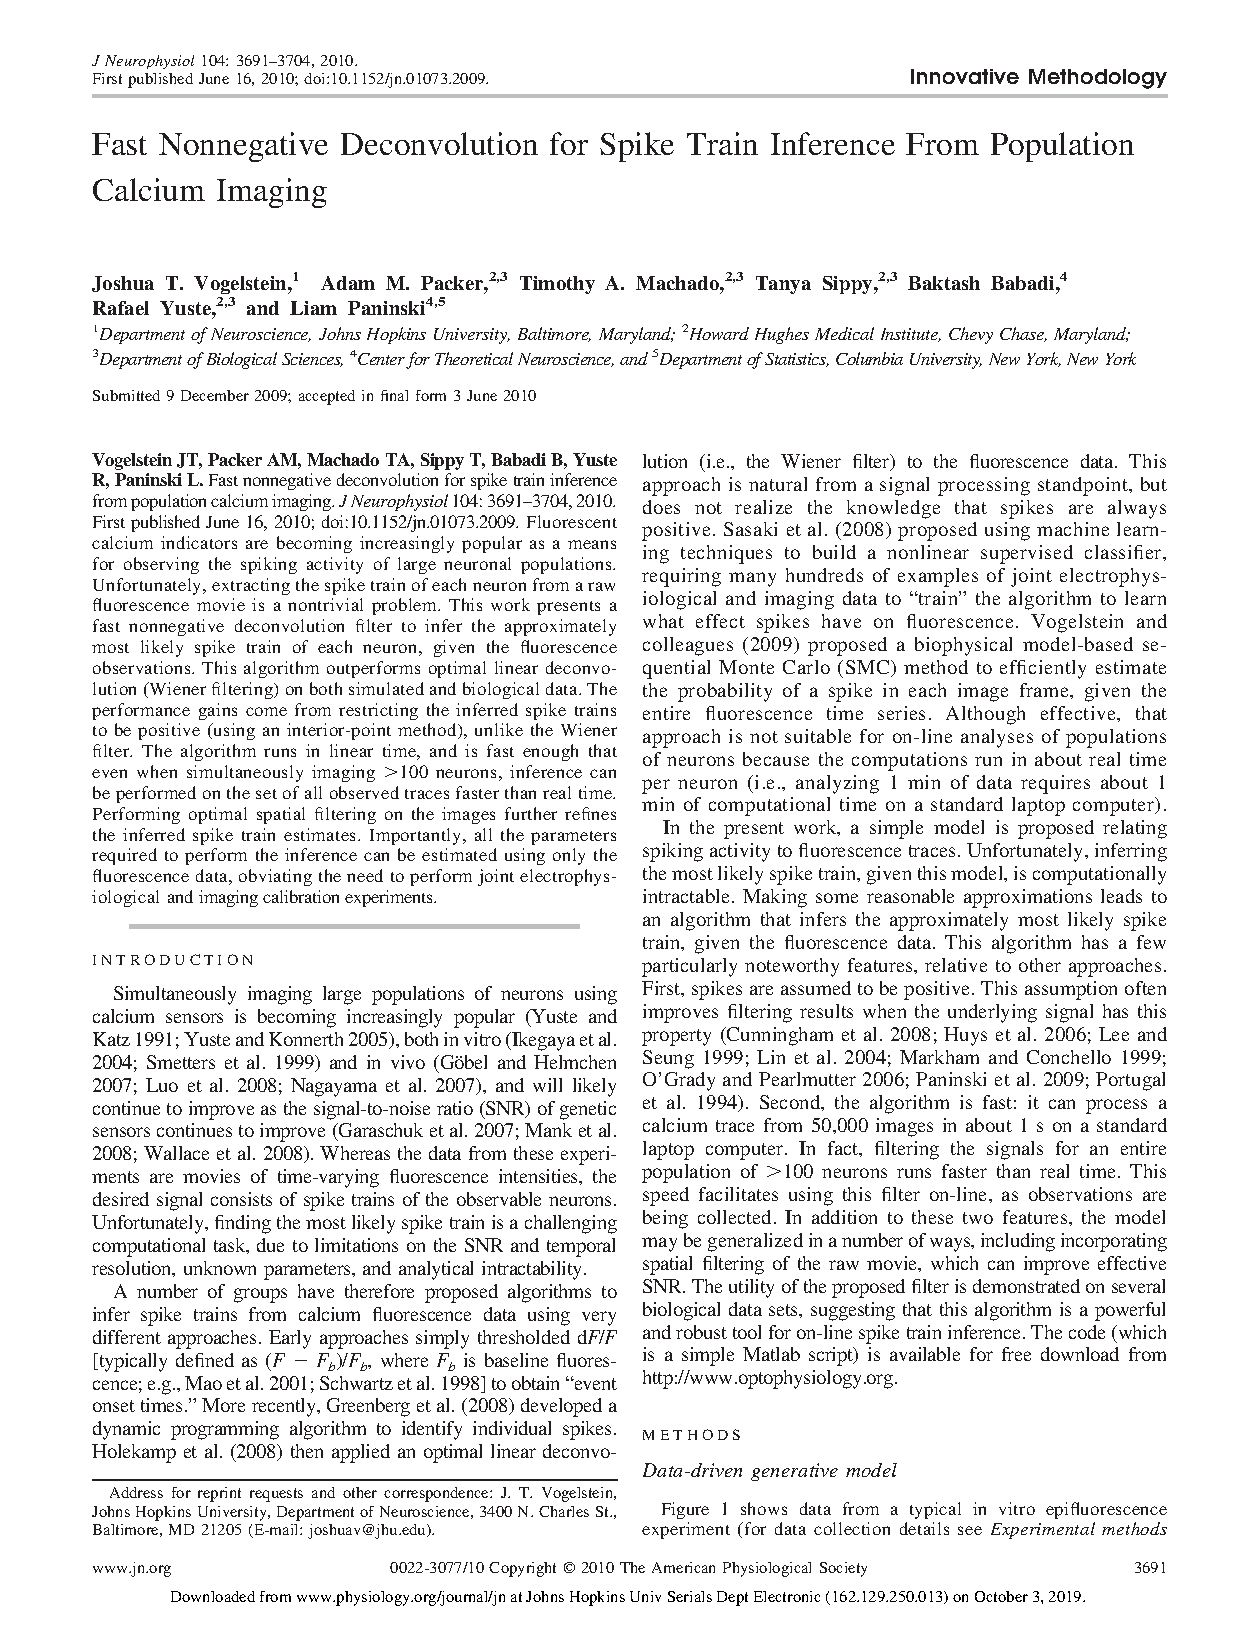
\includepdf[pages=-]{foopsi.pdf}
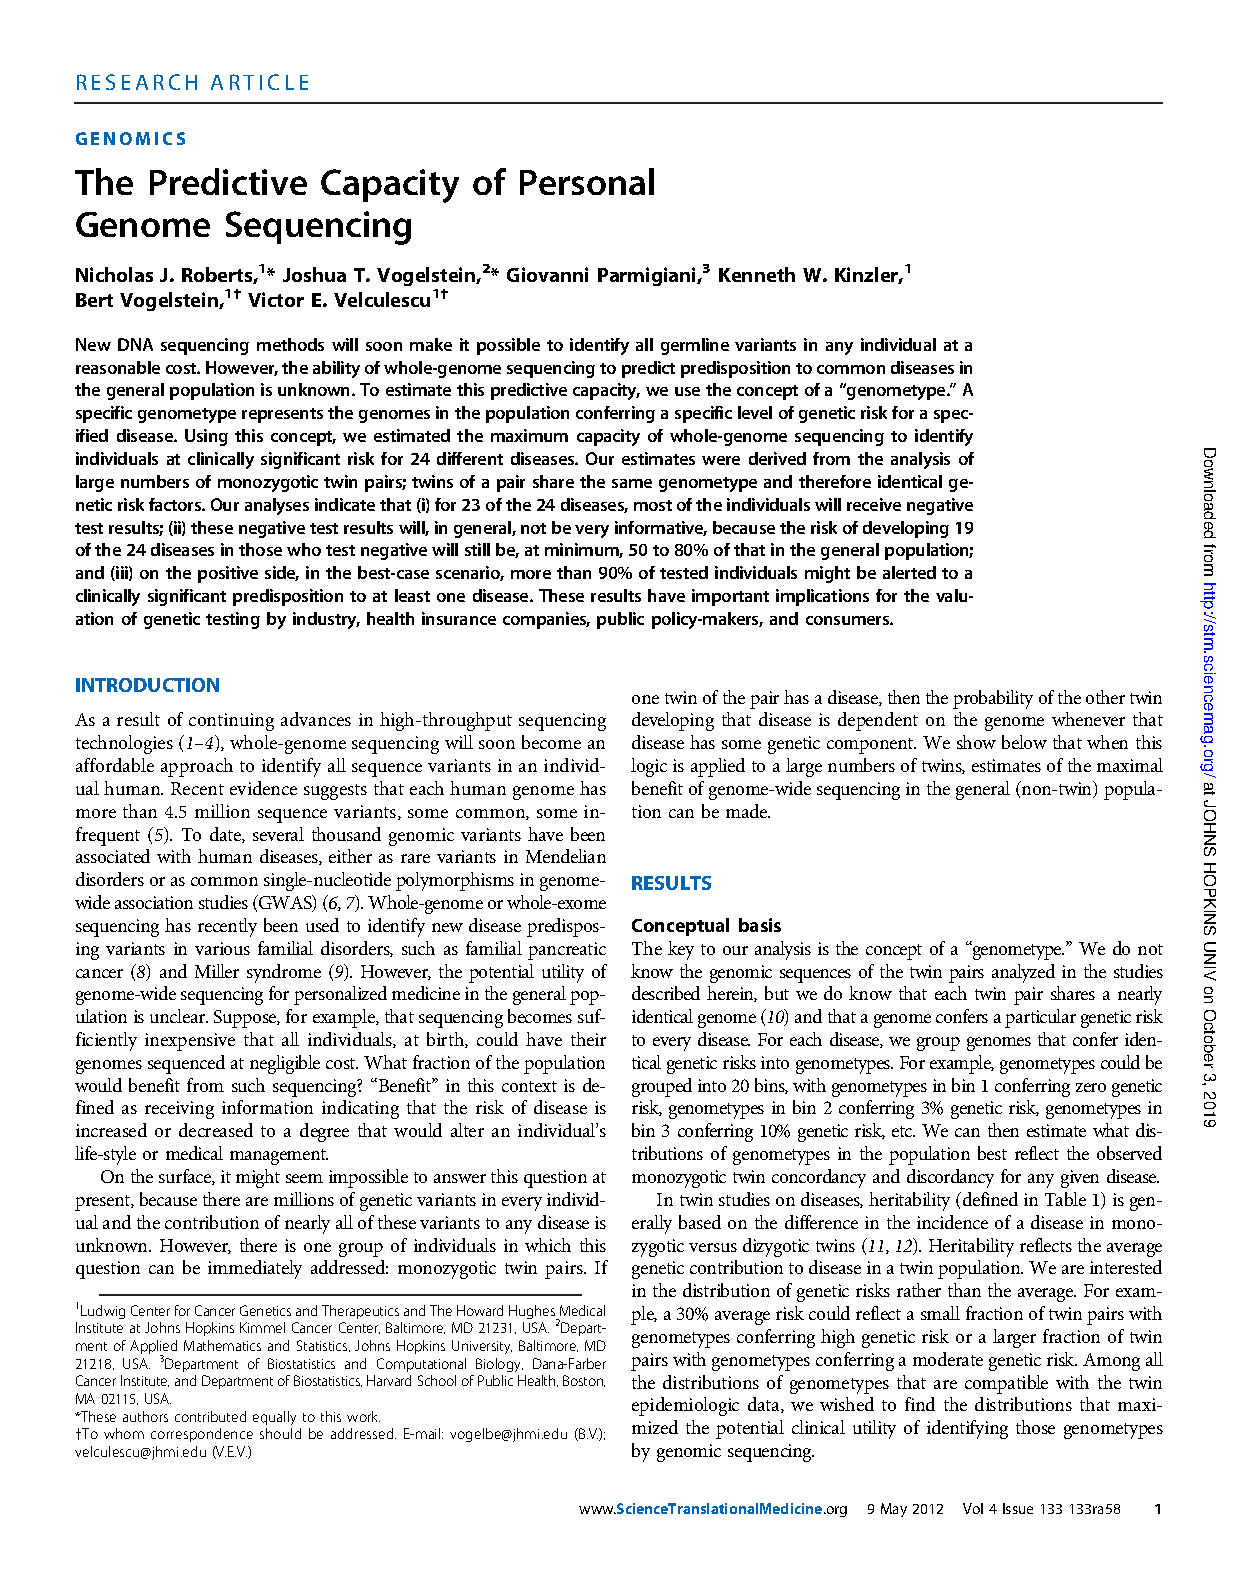
\includepdf[pages=-]{predictive.pdf}
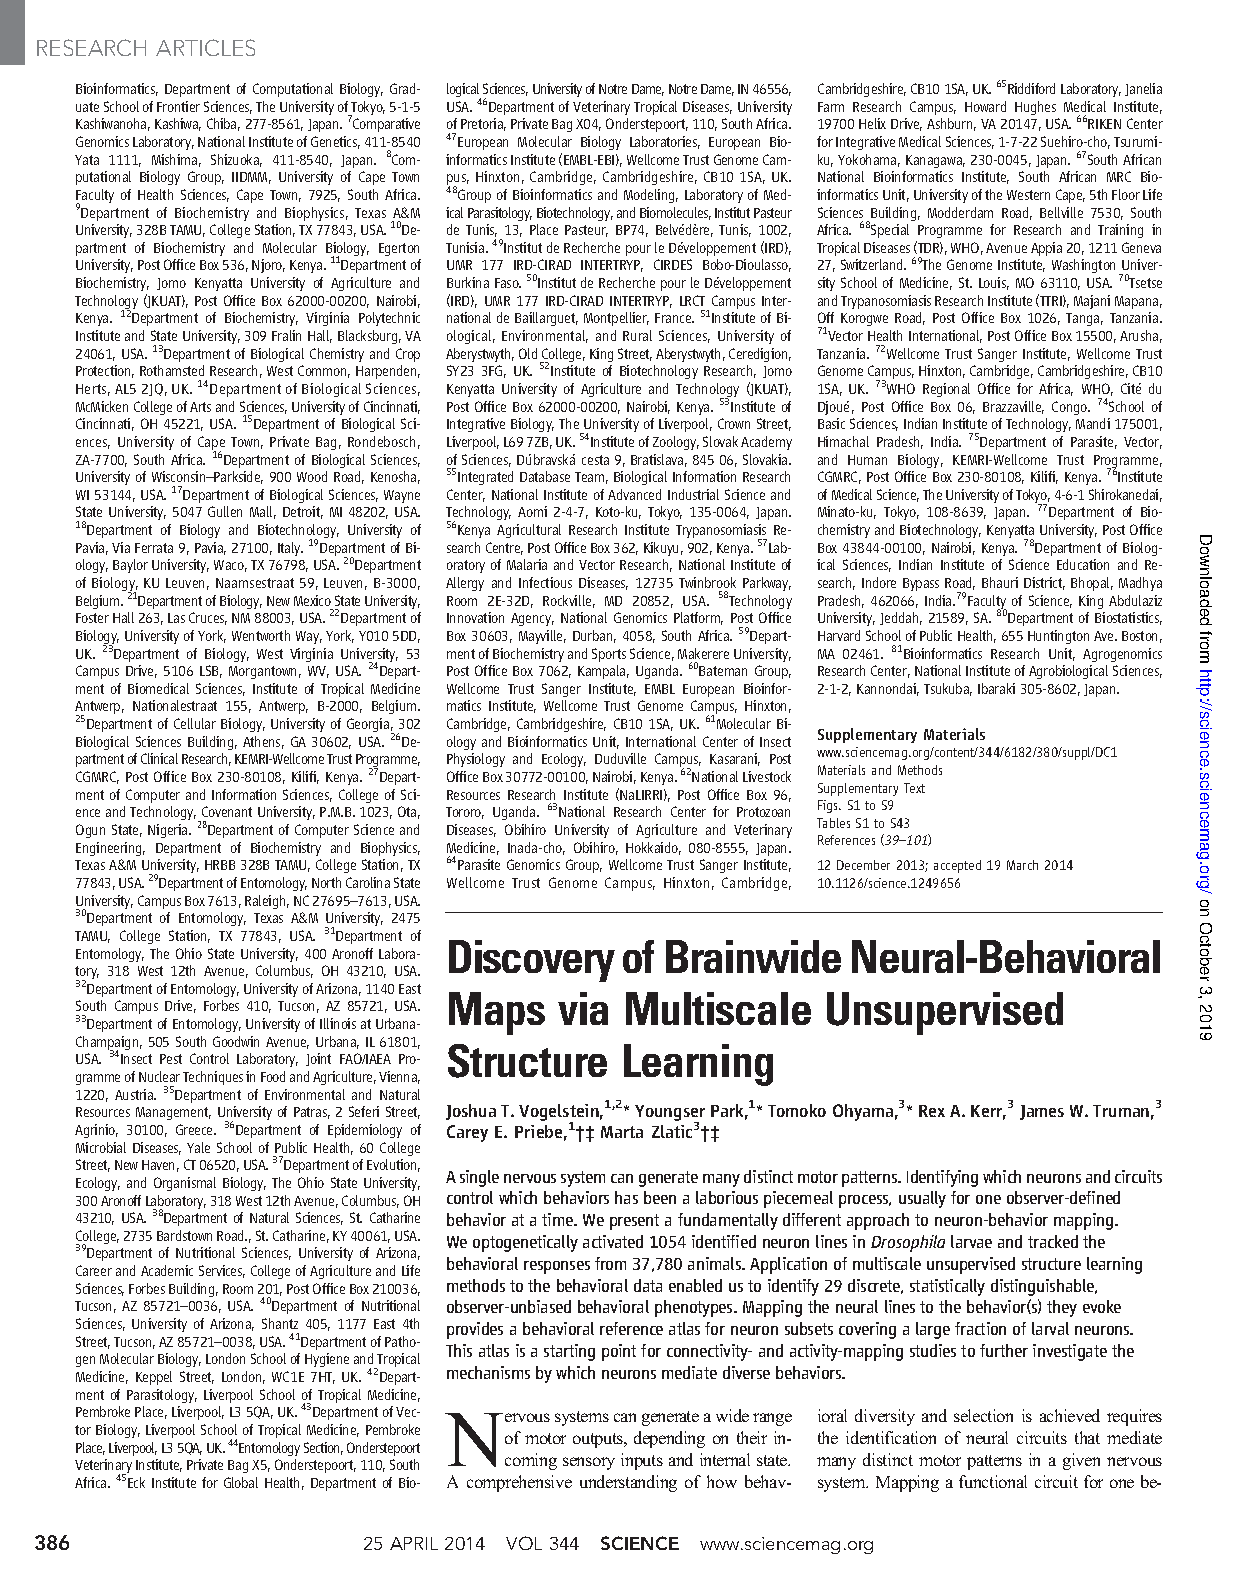
\includepdf[pages=-]{musl.pdf}
\includepdf[pages=-]{ToTheCloud.pdf}


\end{document}
